\begin{figure}[htbp]
    \centering
    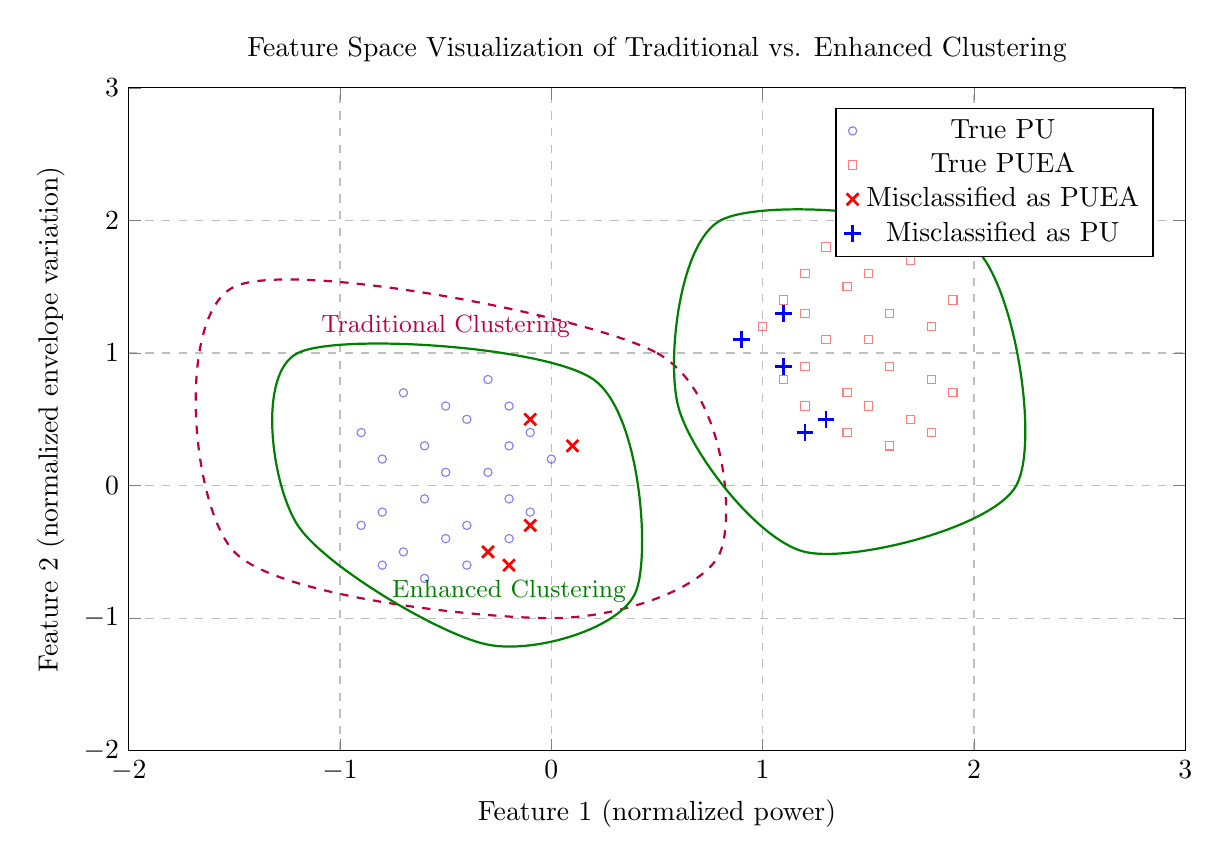
\begin{tikzpicture}
        \begin{axis}[
            width=15cm,
            height=10cm,
            xlabel={Feature 1 (normalized power)},
            ylabel={Feature 2 (normalized envelope variation)},
            xmin=-2, xmax=3,
            ymin=-2, ymax=3,
            xtick={-2,-1,0,1,2,3},
            ytick={-2,-1,0,1,2,3},
            legend pos=north east,
            ymajorgrids=true,
            xmajorgrids=true,
            grid style=dashed,
            title={Feature Space Visualization of Traditional vs. Enhanced Clustering}
            ]
            
            % Original data points
            \addplot[only marks, mark=o, mark size=1.5pt, color=blue, opacity=0.5] 
                coordinates {
                (-0.2,0.3) (-0.5,0.6) (-0.8,0.2) (-0.6,-0.1) (-0.4,0.5) 
                (-0.3,0.8) (-0.7,0.7) (-0.9,0.4) (-0.5,0.1) (-0.1,0.4)
                (-0.2,0.6) (-0.6,0.3) (-0.8,-0.2) (-0.4,-0.3) (-0.2,-0.1)
                (-0.3,0.1) (-0.5,-0.4) (-0.7,-0.5) (-0.9,-0.3) (-0.1,-0.2)
                (0.0,0.2) (-0.2,-0.4) (-0.4,-0.6) (-0.6,-0.7) (-0.8,-0.6)
            };
            \addlegendentry{True PU}
            
            \addplot[only marks, mark=square, mark size=1.5pt, color=red, opacity=0.5]
                coordinates {
                (1.2,1.3) (1.5,1.6) (1.8,1.2) (1.6,0.9) (1.4,1.5) 
                (1.3,1.8) (1.7,1.7) (1.9,1.4) (1.5,1.1) (1.1,1.4)
                (1.2,1.6) (1.6,1.3) (1.8,0.8) (1.4,0.7) (1.2,0.9)
                (1.3,1.1) (1.5,0.6) (1.7,0.5) (1.9,0.7) (1.1,0.8)
                (1.0,1.2) (1.2,0.6) (1.4,0.4) (1.6,0.3) (1.8,0.4)
            };
            \addlegendentry{True PUEA}
            
            % Mislabeled points (with different markers)
            \addplot[only marks, mark=x, mark size=3pt, color=red, line width=1pt]
                coordinates {
                (-0.1,-0.3) (-0.3,-0.5) (0.1,0.3) (-0.1,0.5) (-0.2,-0.6)
            };
            \addlegendentry{Misclassified as PUEA}
            
            \addplot[only marks, mark=+, mark size=3pt, color=blue, line width=1pt]
                coordinates {
                (1.1,0.9) (1.3,0.5) (0.9,1.1) (1.1,1.3) (1.2,0.4)
            };
            \addlegendentry{Misclassified as PU}
            
            % Traditional clustering boundary (less accurate)
            \draw[thick, purple, dashed] plot [smooth cycle] coordinates {
                (-1.5,1.5) (0.5,1) (0.8,-0.5) (0,-1) (-1.5,-0.5)
            };
            \node[purple, font=\small] at (-0.5,1.2) {Traditional Clustering};
            
            % Enhanced clustering boundary (more accurate)
            \draw[thick, green!50!black] plot [smooth cycle] coordinates {
                (-1.2,1) (0.2,0.8) (0.4,-0.8) (-0.3,-1.2) (-1.2,-0.3)
            };
            \node[green!50!black, font=\small] at (-0.2,-0.8) {Enhanced Clustering};
            
            \draw[thick, green!50!black] plot [smooth cycle] coordinates {
                (0.8,2) (2,1.8) (2.2,0) (1.2,-0.5) (0.6,0.6)
            };
            
        \end{axis}
    \end{tikzpicture}
    \caption{Feature space visualization comparing traditional clustering boundary (dashed purple line) with enhanced clustering boundary (solid green line). The enhanced approach reduces misclassifications by adapting to local data patterns.}
    \label{fig:clustering_vis}
\end{figure}
